\section*{Front-End Web Development with React}

This course introduces the React framework, its components, and essential elements like routing, forms, and animations. Shared state management, with the corresponding tools like Redux, is another critical topic covered alongside fetching data.

\subsection*{Single Page Application}
A traditional website is a collection of pages and resources fetched to the server for each page that is navigated. Even if many pages have parts in common, like footer or header, they are requested entirely every time a new page is navigated. In a Single Page Application (SPA), the entire website is downloaded at first, then only the data that changes are re-downloaded from the server. A SPA enables delivering a user experience closer to a desktop application, does not need to be entirely reloaded, and allows the browser to re-render only the changed parts. 
One downside of a SPA is that Search Engine Optimization (SEO) is more difficult to achieve, and the initial page load can be slower than a traditional website.


\subsection*{React Overview}

React is a JavaScript library for building component-based user interfaces using a declarative approach. React focuses only on user interface and is designed for speed, simplicity, and scalability.

A React component is a JavaScript class or function that is imported from the React Module. It is then rendered using the React's rendering function \texttt{ReactCOM.render(...)}.

\subsubsection*{Components}
A component is an independent and reusable set of React elements that should appear on the screen. Every component can accept any input and is composed of React tags that always start with a capital letter and native tags, which start with lowercase letters and are treated as DOM tags.
Every component has a local state which can hold multiple information that can be passed to children components using \texttt{props}. The state is an immutable object that can be updated using the \texttt{setState(...)} directive. This function accepts the property to update and merge it with the actual state. Only class components can have a local state. The state must never be manipulated directly.

Handling event is possible in a similar way as on DOM elements:

\begin{center}
    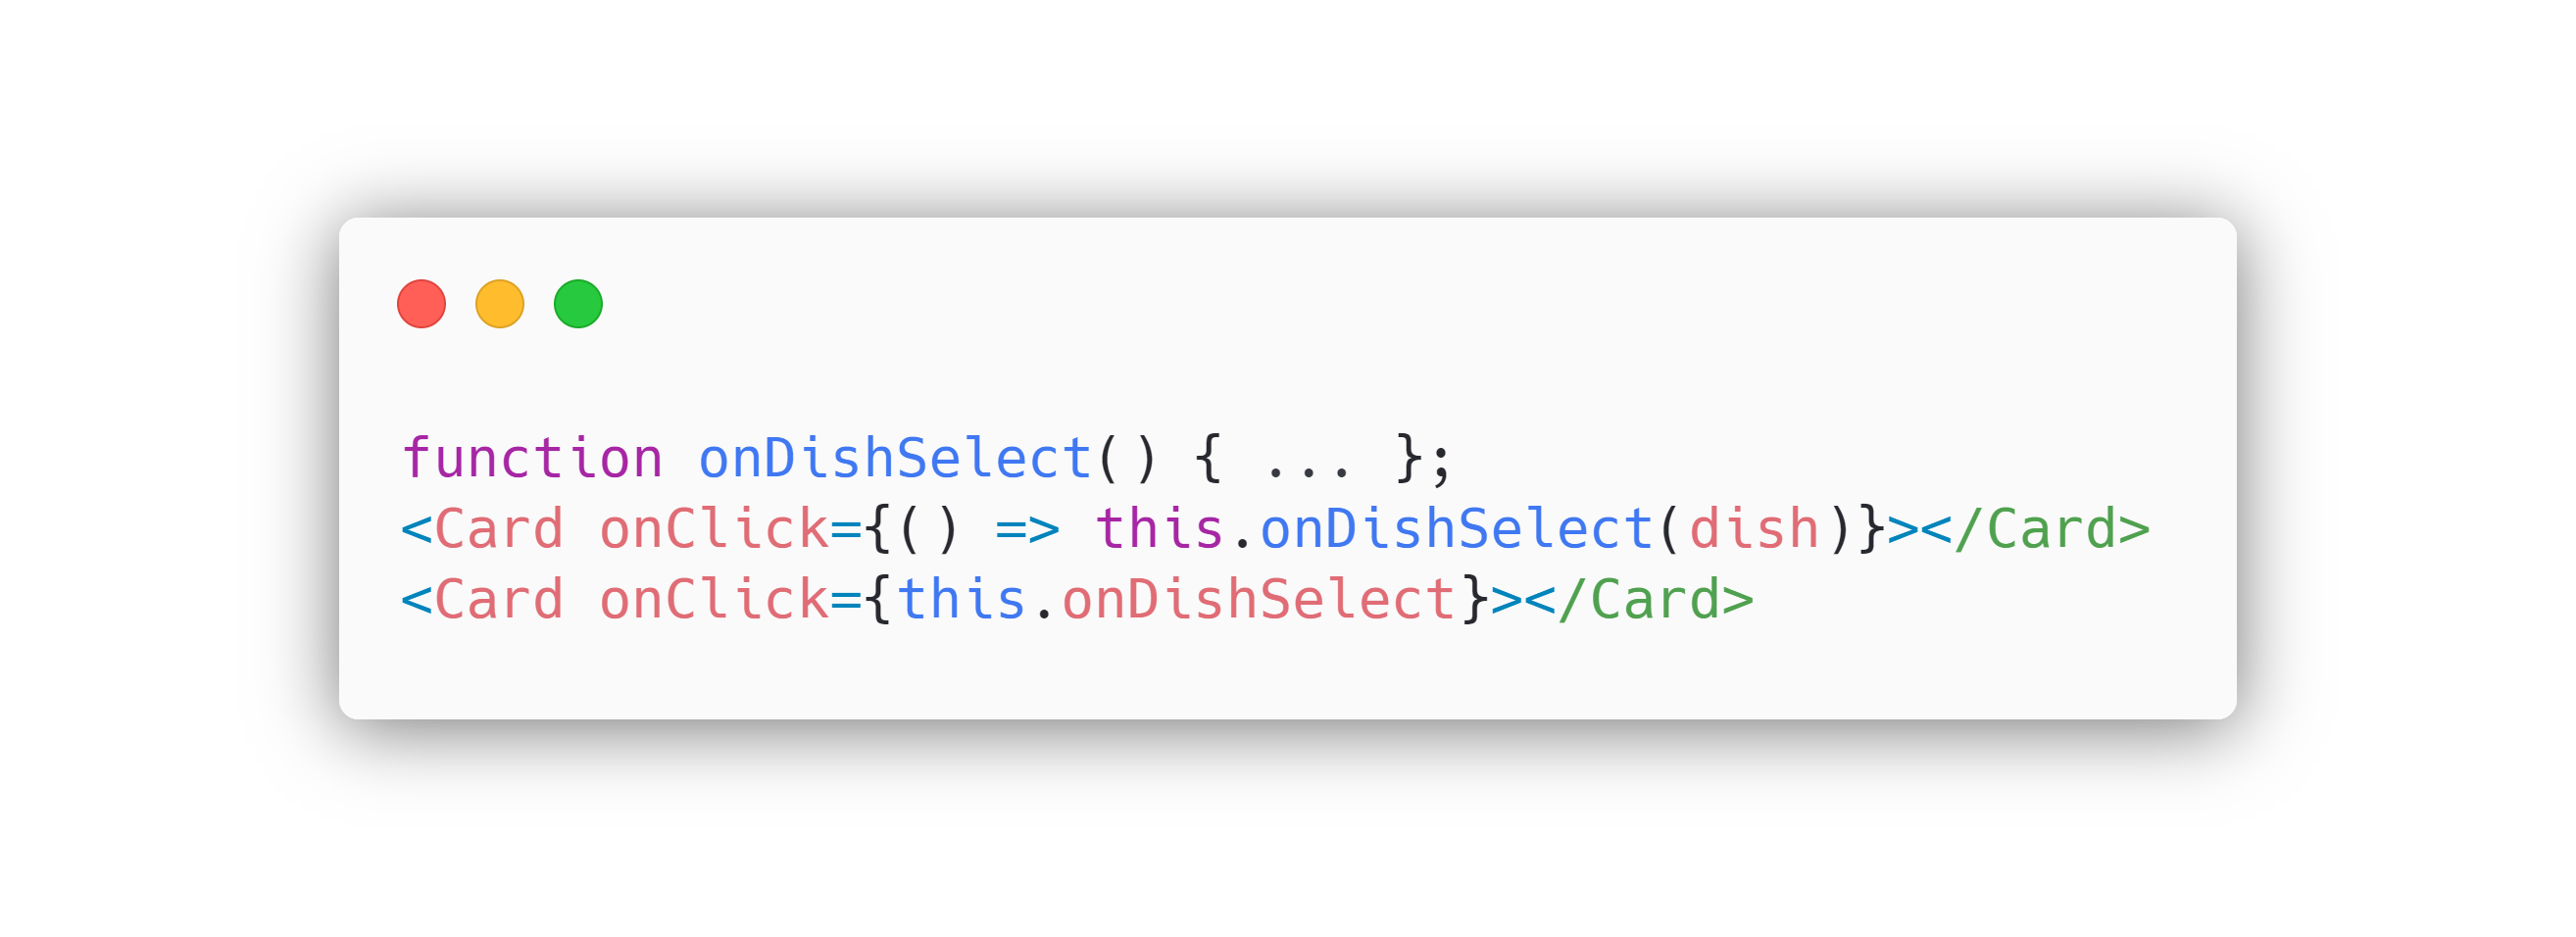
\includegraphics[width=0.8\textwidth]{assets/react-event-handling.png}
\end{center}

In the above figure is possible to see how map a function to a click event on the React element \texttt{Card}.

\subsubsection*{Lifecycle}
React provides life cycle hooks/methods that can be invoked to perform certain operations. A component is created and then mounted in the application, and when it's not required anymore is unmounted. There are three stages of the lifecycle: mounting, updating, and unmounting. Each stage provide, when component is declared as class, several methods like a constructor (mounting), \texttt{componentDidMount()} (called after mounting is finished), \texttt{render()} (call when rendering UI) and many others.

\subsubsection*{Document Object Model}
In the browser, there is an object called \texttt{Browser DOM} (Document Object Model) and is the representation of the structure and data of a webpage. React uses a lightweight version of DOM called \texttt{Virtual DOM}, which uses an in-memory tree data structure of plain JavaScript objects, is extremely fast to manipulate compared to browser DOM and is fully recreated on every setState. 

A diffing algorithm detects which nodes are changed and updates only the minimum number of components in the sub-tree that is updated.

React 16.8 introduced React Hooks to use lifecycle hooks also in a functional component. This topic is not covered in the course but will be discussed in the end of this chapter.

\subsubsection*{Functonal vs Class}
Until the release of \texttt{React 16.8} in 2018, there were two ways of declaring a component: class component or functional component. Functional components are s JavaScript function that returns a React element, can receive props but cannot provide local state or lifecycle hooks. 
\begin{center}
    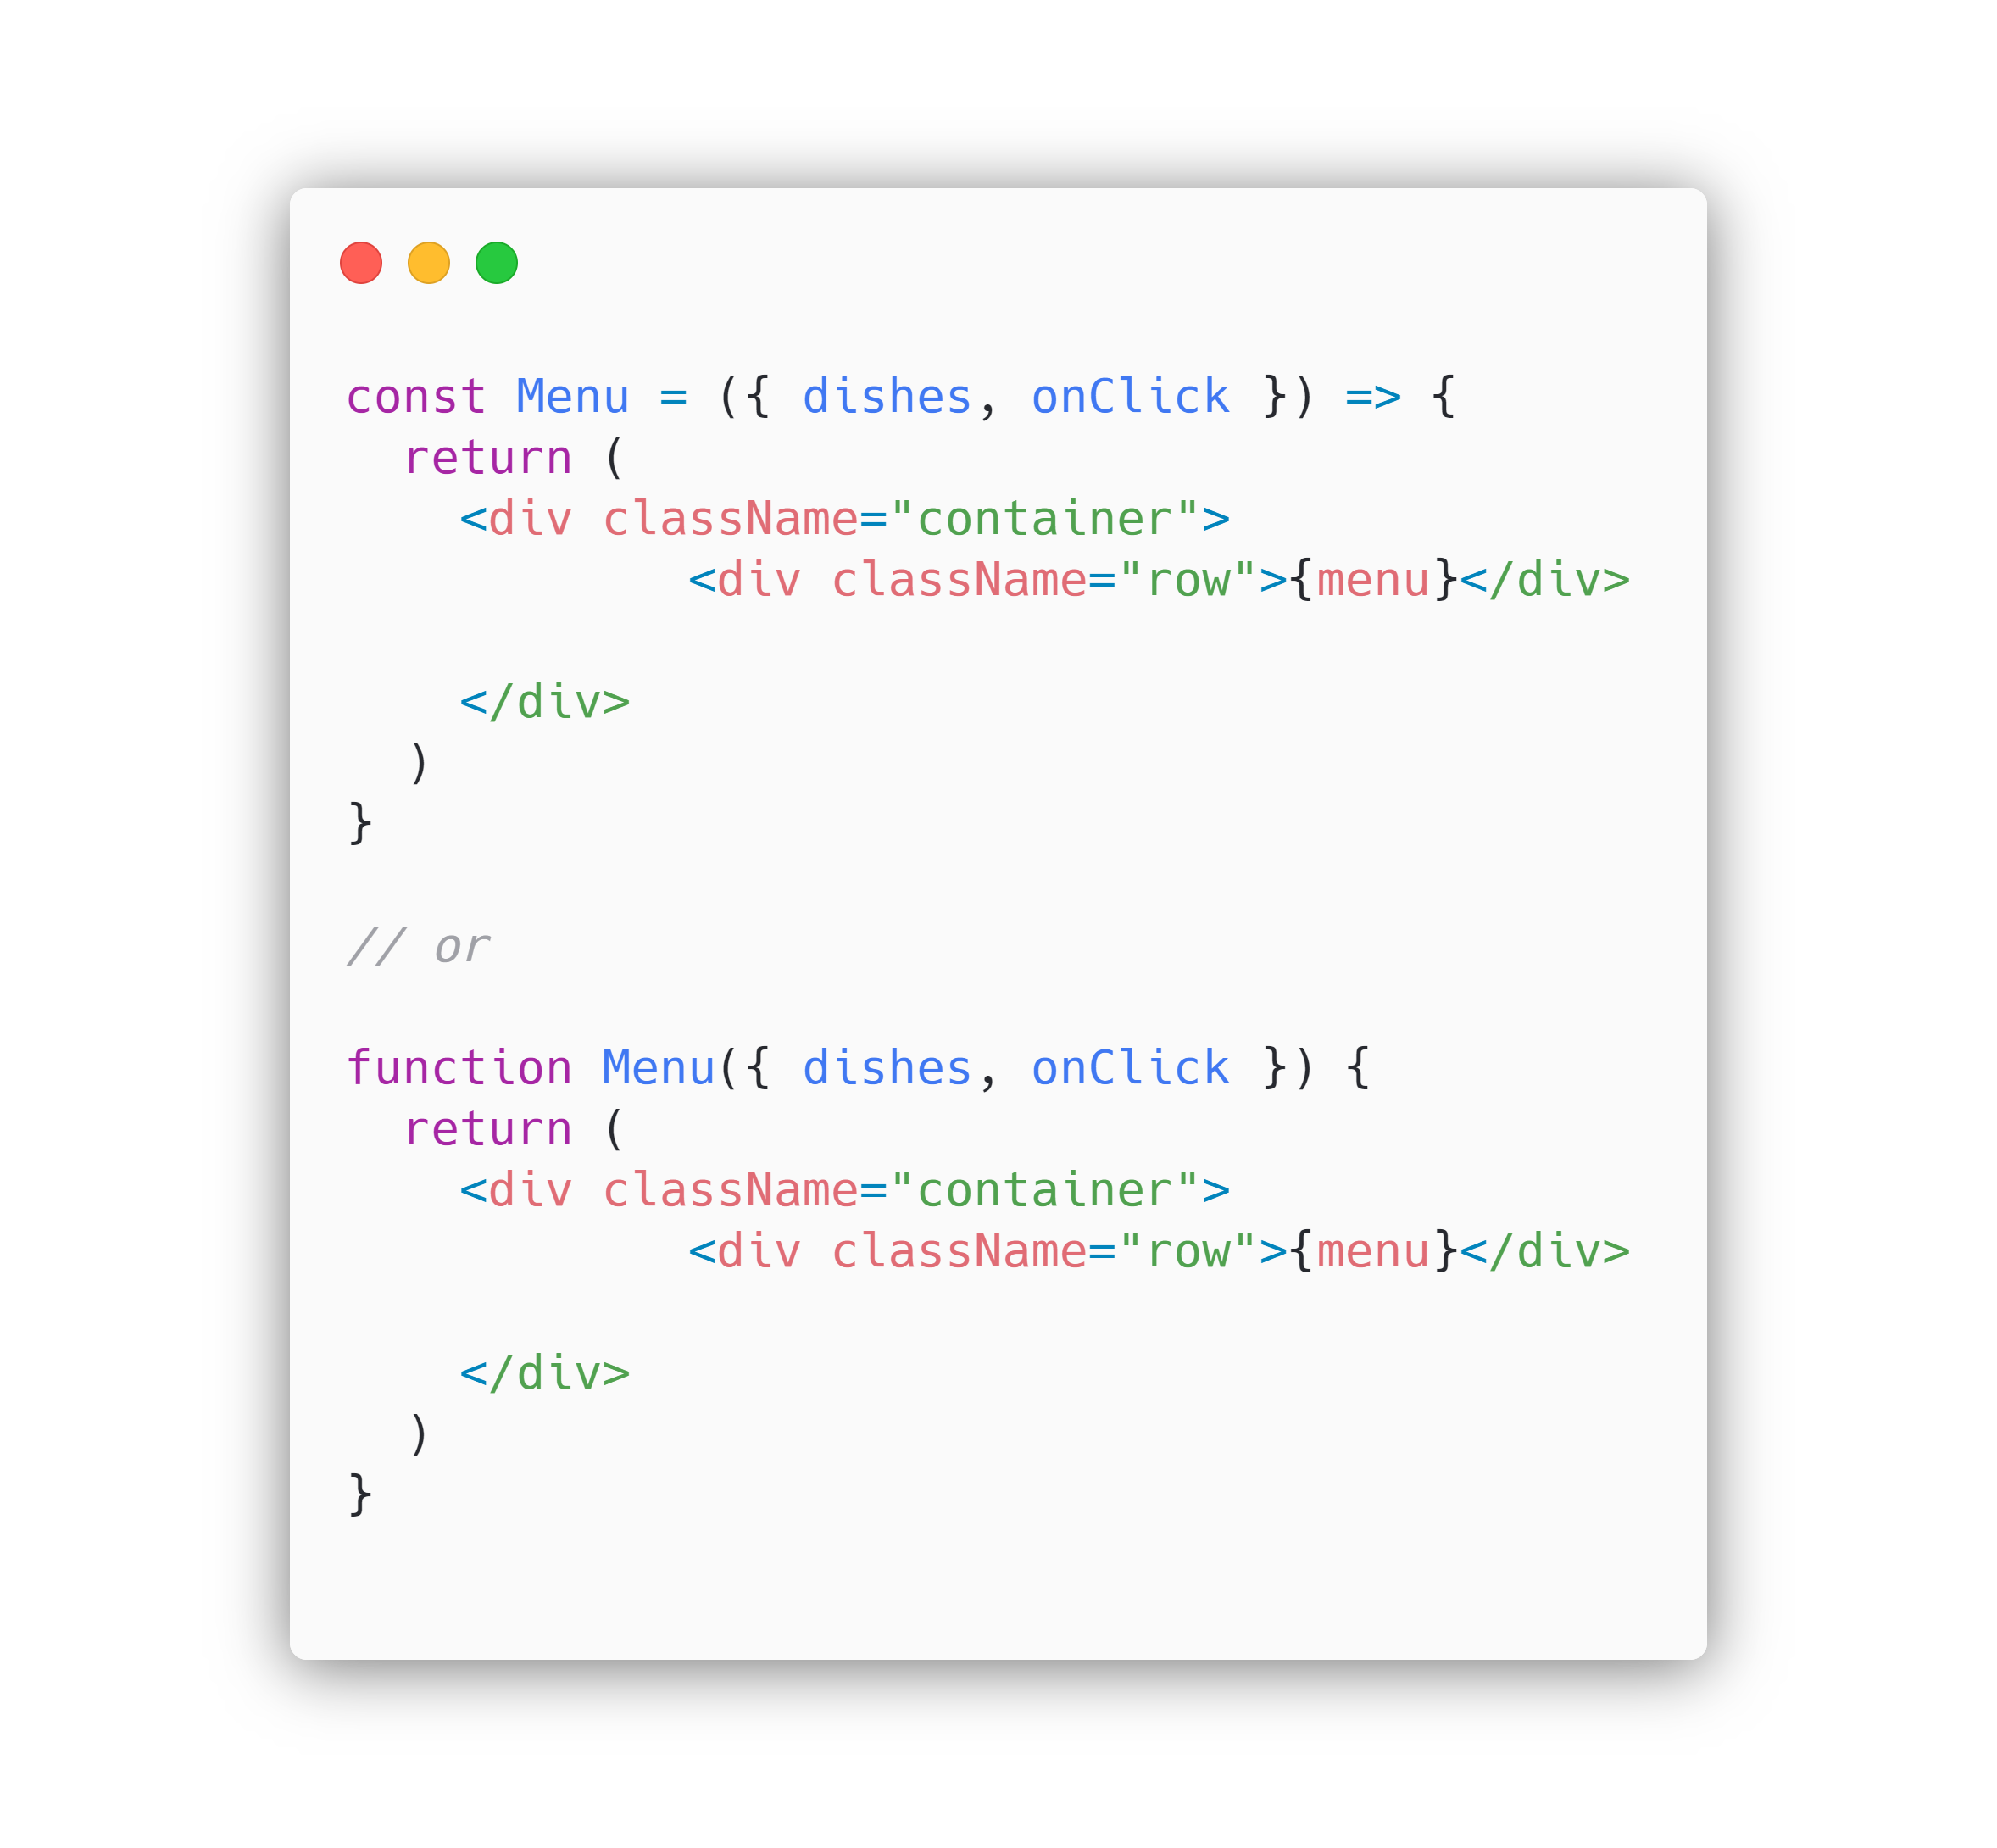
\includegraphics[width=0.8\textwidth]{assets/class-vs-functional.png}
\end{center}

In the above figure is possible to see how a functional component is defined.


\subsubsection*{React Router}
React Router gives the ability to navigate between views using links. It's a module that needs to be additionally installed into the React application called \texttt{react-router-dom}. It is a collection of navigational components that enable navigation among views and support browser-based bookmarkable URLs to navigate in the web app. It is also possible to pass optional parameters.
This dependency allows you to use the \textit{<BrowserRouter>} tag, which enables navigation between multiple pages.
There is also the possibility to use \textit{<Route>} to specify the path to a page or component, or \textit{<Switch>} to group several routers and route the page according to state (like any switch).
Navigation is possible using \textit{<Link>} or \textit{<NavLink>}.

\subsubsection*{Parameters}
It is possible to pass parameters through the URL and pass it to the view. For example \textit{/menu/42} can be rendered in the view mapped to \textit{/menu} with an input parameter \textit{42}.

\subsubsection*{Forms}
In React, there are two types of forms: controlled or uncontrolled.
Controlled forms are directly and bidirectionally tied to the state, and every state mutation is associated with a handler.

An uncontrolled form is not tied to the state but holds the values internally in the DOM. It is possible to retrieve data, for example, when sending information to a REST API and does not need to have a handler for every state update.


\subsection*{MVC Framework}
A Model-View-Controller is an architectural pattern commonly used to allow reusable components, isolate logic from user interface and permit independent development, testing, and maintenance. 
The \textit{Model} part usually is used to manage behavior and data, respond to requests about state or instruction to change state, and notify the View when there is a change in the state.
The \textit{View} is used to present the information in the user interface.
A \textit{Controller} receives the input from the users, instructs the Model on which action to perform, and initiates a response.

React is not a complete MVC framework (or its descendent Model-View View-Model). It only provides the presentation logic. The Model and Controller can be developed independently from the View using React.

\subsection*{Flux and Redux}
The Flux architecture is an alternative to the MVC approach. It is a unidirectional data flow, from an action to the view through a dispatcher and a store.
All updates have one unidirectional flow, and the central unit is the store. If a view wants to update the store, it must use an action. It cannot modify the store directly.
New action is propagated through the systems in response to user interaction, and the dispatcher controls all the changes made to the store.

\subsubsection*{Redux}
Redux is the place to store the application's state and allow to have a consistent way to access it. Redux is widely adapted by the React community but is not strictly connected to React itself. Redux makes state mutations predictable.
The state is a single object and is the single source of truth, it is read-only, and the only way to change the state is through actions. Every change must be made with pure functions that take the previous state and return a newly mutated one.
Using Redux is possible to implement logging utilities, API handling, undo/redo of a state, and many other features.  
The store holds the current state value as a plain JavaScript object. There are some utilities provided from Redux to manage the store:
\begin{itemize}
    \item \textit{createStore} - method that allow to create a store with an initial state
    \item \textit{dispatch} - update the state with the provided action object
    \item \textit{subscribe} - accepts a callback function that will be run every time an action is dispatched
\end{itemize}

The bindings between React and Redux are possible using the package \textit{react-redux}. It will provide a function \textit{connect()} that generates a wrapper container that subscribes to the store. It takes two additional arguments:
\begin{itemize}
    \item \textit{mapStateToProps()} - called every time the store state changes. Return an object full of data with each field being a prop for the wrapped component
    \item \textit{mapDispatchToProps()} - eceives the dispatch() method and should return an object full of functions that us dispatch()
\end{itemize}

Surrounding the React App with a tag <Provider> allows to provide the store as an attribute and make it accessible as a singleton to all the connected components.

\subsubsection*{React-Redux-Form}\textit{React-readux-form} is a versatile, fast, and intuitive library for creating complex and performant forms in React using Redux, providing a collection of reducer and action creators. Form data are stored in a Redux store in a model. It is suitable to use when there is a need to persist form data across the component lifecycle.

\subsubsection*{Redux Actions}
Redux Actions are payloads of information that are sent, through \textit{store.dispatch()} from your application to the store to effect any change in the store's ticket. Every action should have a property \textit{type}, usually a constant string, and a payload containing all the data necessary for updating the state.

\subsubsection*{Reducers}
A reducer is a function that takes the previous and the data that should be updated. The last state is copied and merged with the data to create the next state. A reducer should never mutate directly the state.

\subsection*{Redux Middleware and Thunk}
The Redux Middleware can run a code after an action is dispatched and before it reaches the reducer. It is a place that enables third-party extensions to be injected into your Redux application. For example, suppose the developer wants to log all the actions that have been dispatched. In that case, a middleware is a good point to capture the action, log what the action is, then let it move on to the reducer, and then log the application's state after the action is effected.

Middleware forms a pipeline that wraps around the dispatch(). Then it can make any modification and pass the action forward (pass-through). It can restart the dispatch pipeline and also access the store state.
Is it helpful for: inspecting the actions and the state, modify actions, dispatch other actions or stop actions from reaching the reducers.
It is used with applyMiddleware() that sets up the middleware pipeline and returns a "store enhancer" that is passed to createStore().

\subsubsection*{Thunk}
A subroutine is used to inject an additional calculation in another subroutine: delay a calculation until its results are needed or insert operations at the beginning or end of the other subroutine.
Middleware allows writing action creators that return functions instead of an action. For example, it can be used to delay the dispatch of an action or dispatch only if a particular condition is met.

The inner function receives the \textit{dispatch()} and \textit{getState()} store methods. The state can be examined and decide if it allows the action to proceed. Is it useful for complex synchronous logic like multiple dispatches, conditional dispatches, or simple async logic.

\subsubsection*{Fetching Data}
Since React is focused only on the view, it is possible to handle data fetching in multiple ways. The fetch API, a replacement for the old XMLHttpRequest, is the most commonly used fetching resource that provides a promise-based interface.

\subsection*{Animations}
There were two libraries when the course was delivered, which were widely used for animations:
\begin{itemize}
    \item \textit{react-transition-group}
    \item \textit{react-animnation-components}
\end{itemize} 
The last update in \textit{react-animnation-component} is dated 04 April 2018 and, because of that, was skipped during this course.
On the other hand, \textit{react-transition-group} is still widely used and maintained. It provides a set of components for managing component states (including mounting and unmounting) over time, specifically designed with animation in mind. The most common components are <Transition>, <CSSTransition>, and <TransitionGroup>.
A Transition is used to describe the transition from one component to another with some states: entered, exiting, or exited. It is used to animate the mounting and unmounting of a component. A set of <Transition> components can be grouped in a list using the <TransitionGroup> tag.
CSSTransition is applied together with <Transition>. It applies a pair of class names during the transition's appear, enter, and exit stages. It also uses props to decide when to apply the transition classes 


\subsection*{React Hooks}
React Hooks were not covered in the course, but since they are a significant change made by React 16.8, I decided to go over them anyway.
Hooks have radically changed how development is done in React, making class-defined components obsolete in favor of functional components.

Hooks provide some functions that allow for manipulating the internal state of functional components. For example, the useState() function permits the insertion and manipulation of the state within a component.

\begin{center}
    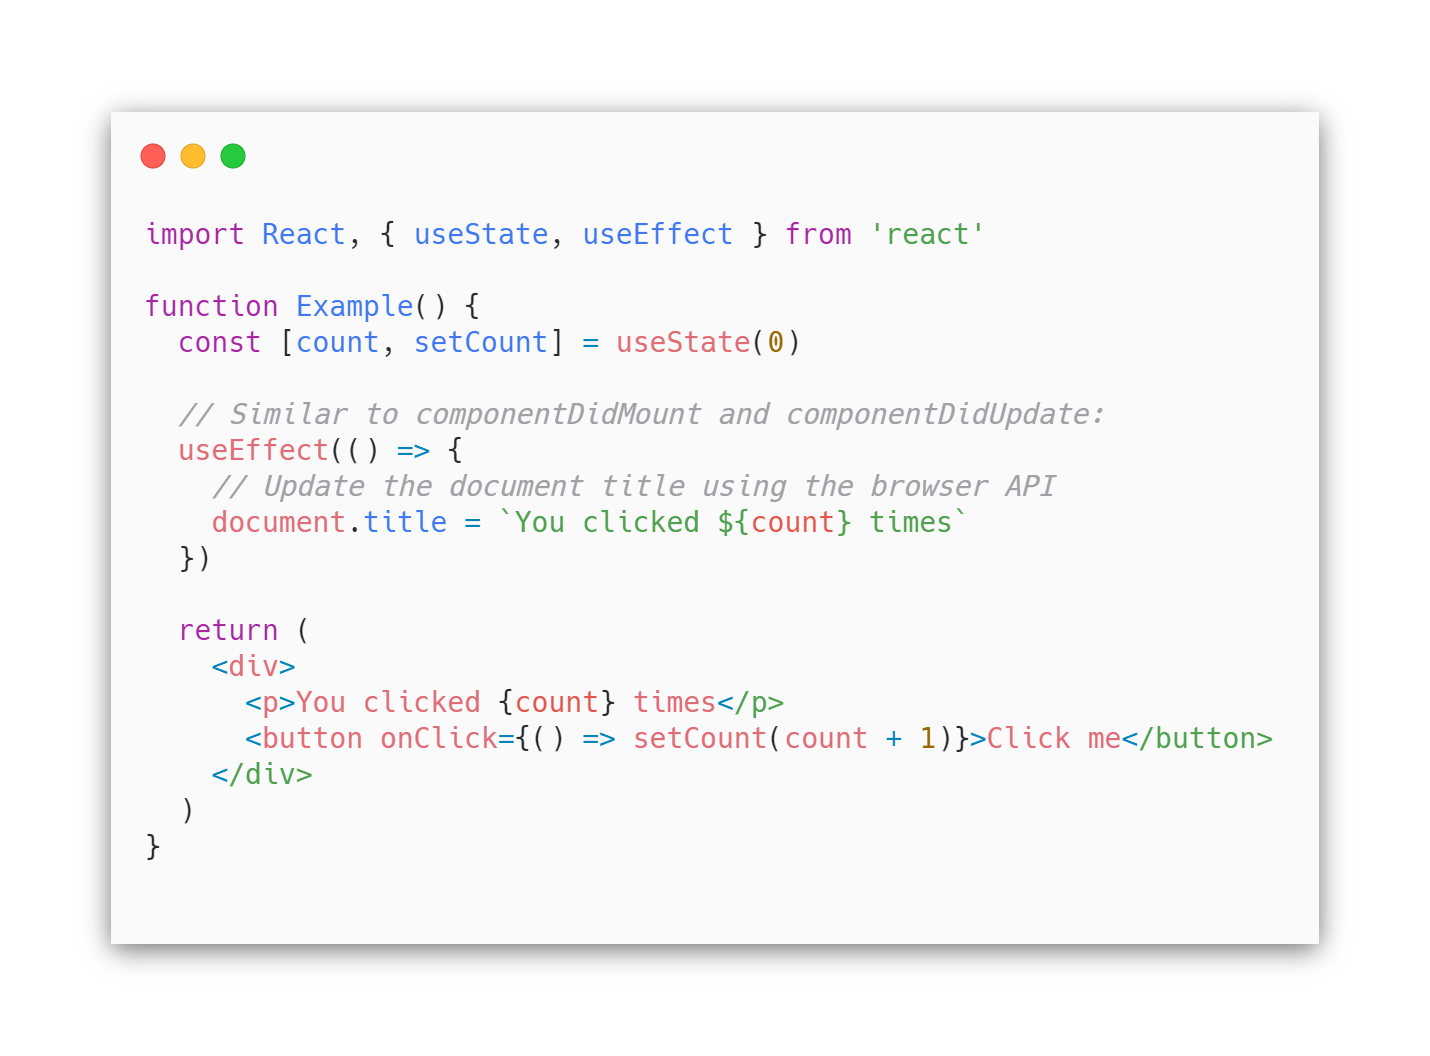
\includegraphics[width=0.8\textwidth]{assets/hooks.png}
\end{center}

useEffect is another important hook that allows manipulating the state during the lifecycle of the component. It replaces the componentDidMount, componentDidUpdate and componentWillUnmount functions with a single function. It is possible to cause the component to render when one or more parts of the state are changed and define its custom hooks. Hooks can only be used by a component at the top level, not within loops or conditions.